% chapters/glitch.tex
%
% Copyright 2023 Alexander Lyttle.
%
% This work may be distributed and/or modified under the conditions of the
% LaTeX Project Public License (LPPL) version 1.3 or later.
%
% The latest version of this license is in
% https://www.latex-project.org/lppl.txt and version 1.3 or later is part of
% all distributions of LaTeX version 2005/12/01 or later.
%
%
\chapter[Acoustic glitches]{Acoustic glitches as a signature of helium abundance}\label{chap:glitch}

A glitch arises from a sharp structural variation in the star.

Explain that glitches can be a signature of helium abundance. If we can model the glitch consistently between models and observed stars, we can add parameters to the HBM which contain information about helium.

In this chapter, we explore the theoretical background of acoustic glitches

\section{Theory of the glitch}

\subsection[1D example]{A one-dimensional example of a glitch}

A rapid variation in the structure of a medium induces an oscillation in the eigenfrequencies, \(\delta\omega\) . To demonstrate this, we consider a simple one-dimensional example. Consider a medium bound from \(x=0\) to \(x=L\) in which pressure waves can propagate at speed \(c\). The longitudinal displacement of the wave \(\xi\) must obey the wave equation,

\begin{equation}
    \frac{\partial^2\xi(x, t)}{\partial t^2} = c^2 \frac{\partial^2\xi(x, t)}{\partial x^2},
\end{equation}

at any given time \(t\). If \(c\) is constant, the solution to the wave equation is,

\begin{equation}
    \xi(x, t) = r \sin k x \cos(\omega t + \phi),
\end{equation}

where \(r\) and \(\phi\) are the amplitude and temporal phase of the wave. Solutions for \(\omega\) which satisfy \(\xi(L, t)=0\) may be derived as,

\begin{equation}
    \omega_n = c \frac{n \pi}{L},
\end{equation}

where \(n\) is a non-zero integer (the \(n=0\) solution would give \(\xi=0\) everywhere).

where \(\omega\) is the angular frequency and \(k\) is the wave-number, such that \(\omega = c k\).

\begin{figure}
    \centering
    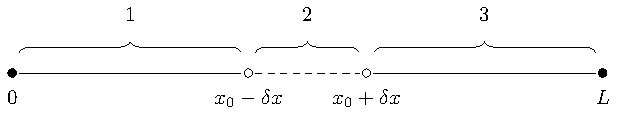
\includegraphics{figures/glitch-1d-example-diagram.pdf}
    \caption[A diagram showing a one-dimensional medium with a small structural perturbation.]{A diagram showing a one-dimensional medium split into three regions. 1: Fixed at \(x=0\) with a constant speed of sound \(c_0\); 2: A small structural perturbation starting at \(x=x_0\) with width \(\delta x\) with constant speed of sound \(c + \delta c\); 3: Fixed at \(x=L\) with a constant speed of sound \(c\).}
    \label{fig:1d-diagram}
\end{figure}




\subsection{Helium glitch}\label{sec:helium-glitch}

Where does the helium glitch come from?

How Tassoul's asymptotic approximation assumes adiabatic exponent of 5/3 but this is not correct for a star. In a star, gamma is effected by the ionisation of elements. This effects the speed of sound,

\begin{equation}
    c = \sqrt{\gamma \frac{p}{\rho}},
\end{equation}

where \(p\) is pressure, \(\rho\) is density, and \(\gamma\) is the first adiabatic exponent,

\begin{equation}
    \gamma \equiv \Gamma_1 = \left( \frac{\partial \ln p}{\partial \ln \rho} \right)_s,
\end{equation}

where \(s\) is specific entropy.

We can simplify the problem to consider a star of just hydrogen and helium. Using the approach of Houdeyer we can derive an apporximation for \(\gamma\) in terms of temperature and density in the star

Reference Houdeyer's paper with plots to show the depression in the first adiabatic exponent with temperature and pressure. 

\begin{figure}
    \centering
    \includegraphics{example-image-a}
    \caption{Multi-panel figure showing \(\gamma\) as a function of \(\rho\) and \(T\) for different values of helium abundance.}
    \label{fig:gamma-temp-density}
\end{figure}

Now we look at the radial order kernels and how they are sensitive to different region


One approach is in Houdek and Gough, to take a perturbation in gamma and propagate this to a perturbation in frequency.

\subsection{Base of the convective zone glitch}\label{sec:bcz-glitch}

Other glitches are present. Sharp structure variation

\section{Modelling glitches in stellar oscillations}


\subsection{Gaussian processes }\label{sec:glitch-gp}

